\section{Implementación de tabla de verdad con compuertas lógicas}

\vspace{2mm}
\begin{wraptable}{r}{5cm}
    \begin{center}
        \begin{Karnaughvuit}
            \maxterms{0,2,3,7}
            \minterms{1,4,5,6}
            \implicant{1}{5}{green}
            \implicantcostats{4}{6}{blue}
            %\implicant{4}{5}{red}      //para el caso de hazards
        \end{Karnaughvuit}
        \caption{Mapa de Karnaugh de menor costo.}
        \label{fig:mapaKarnaughConGlitches}
        % \caption{Tabla de verdad de la función dada.}
        % \label{wrap-tab:tabladeverdad}
        % \vspace{2mm}
        % \begin{tabular}{c|c|c|c}
        %     a& b & c & $f~(a,~b,~c)$ \\\hline
        %     0& 0 & 0 & 0 \\
        %     0& 0 & 1 & 1 \\
        %     0& 1 & 0 & 1 \\
        %     0& 1 & 1 & 1 \\
        %     1& 0 & 0 & 0 \\
        %     1& 0 & 1 & 1 \\
        %     1& 1 & 0 & 0 \\
        %     1& 1 & 1 & 0 
        % \end{tabular}
    \end{center}
\end{wraptable} 
\par
El objetivo fue implementar la tabla de verdad con compuertas lógicas discretas. 
Se sabe que simplificando ya sea con máxterminos o mintérminos se llega a la expresión mínima, es decir a la máxima simplificación; 
por lo que se procedió a simplificar con mintérminos, resultando en lo siguiente, acorde al mapa de Karnaugh \ref{fig:mapaKarnaughConGlitches}:
\vspace{4mm}
\begin{equation}
    Y=\overline{A}B+\overline{B}C
    \vspace{5mm}
\end{equation}
La expresión anterior es la que representa el menor costo pues se implementa con la menor cantidad posible de compuertas (ver figura \ref{fig:circuito-con-glitches}).
Sin embargo, se observa que al transicionar entre los grupos $(A,~B,~C)=(0,~1,~1)$, -en verde-, y $(A,~B,~C)=(0,~0,~1)$, -en azul-, es decir variando el estado de la variable B, el comportamiento será incierto, pues no está cubierta por ningún mintérmino.
Para medir ésto, se conectó la entrada A a masa, y C, a +Vcc (5~V). La señal B se simuló con una onda cuadrada generando 
así la transición entre los susodichos estados. Esto se puede ver en la figura \ref{fig:glitch}; la entrada es la señal amarilla, y la verde la salida, que se encuentra en un nivel de tensión alto, es decir un 1 lógico, como era de esperar. 
Por otro lado, cuando B varía de 5 V a 0 V, se observa un comportamiento indeseado, un glitch, que se debe a los tiempos de delay propios de las compuertas lógicas.

\vspace{5mm}
\begin{figure}[H]
    \begin{minipage}{.49\linewidth}
        \centering
        \vspace{10mm}
        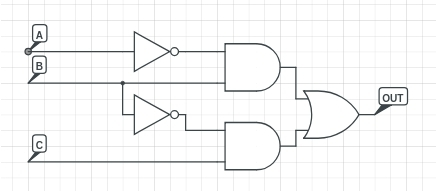
\includegraphics[width=.8\linewidth]{./circconglitches.jpg}
        \vspace{10mm}
        \caption{Circuito utilizado de menor costo.}
        \label{fig:circuito-con-glitches}
    \end{minipage}
    \begin{minipage}{.5\linewidth}
        \centering
        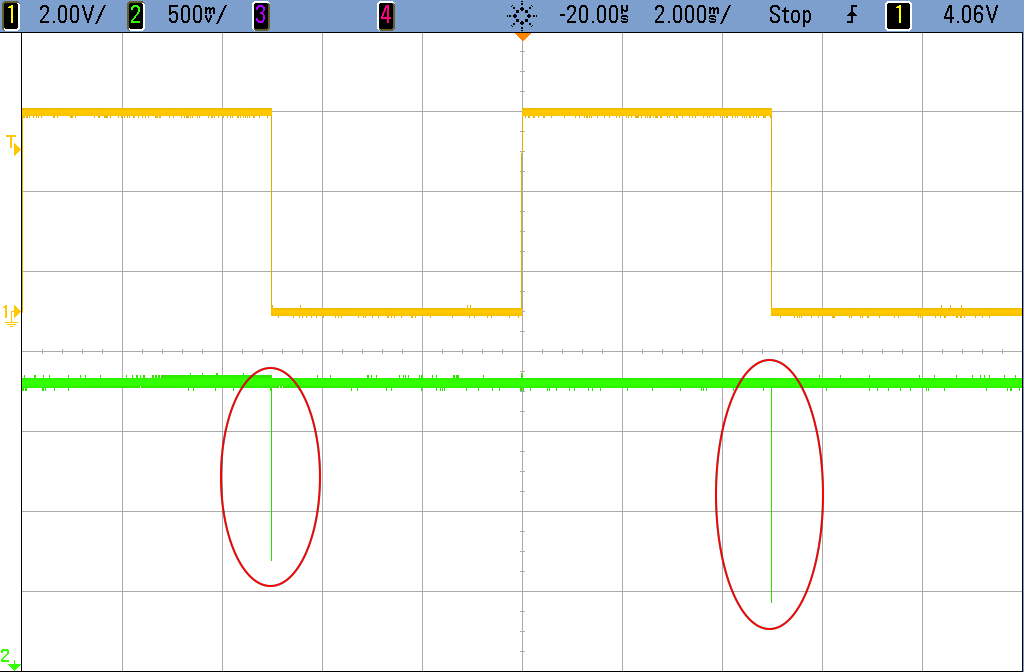
\includegraphics[width=\linewidth]{./glitch.png}
        \caption{Glitch observado señalado en rojo al variar el estado de B.}
        \label{fig:glitch}
    \end{minipage}
\end{figure}

\vspace{5mm}
Para evitar este incoveniente lo que se puede hacer es agregar un grupo al mapa de Karnaugh entre los estados problemáticos, 
para asegurarse que la salida, al transicionar entre los mismos, se mantenga siempre en el mismo valor; ver figura \ref{fig:mapaKarnaughSinGlitches}.
Entonces, agregando un mintérmino, la función queda simplificada a:
\vspace{4mm}
\begin{equation}
    Y=\overline{A}B+\overline{B}C+\overline{A}C
    \vspace{5mm}
\end{equation}

Lo que da como resultado el circuito \ref{fig:circuito-sin-glitches}, que si bien requiere una compuerta más (un OR); y además un AND de tres entradas, evita que haya glitches.

\vspace{5mm}
\begin{figure}[H]
    \begin{minipage}{.49\linewidth}
        \begin{center}
        \vspace{10mm}
        \begin{Karnaughvuit}
            \maxterms{0,2,3,7}
            \minterms{1,4,5,6}
            \implicant{1}{5}{green}
            \implicantcostats{4}{6}{blue}
            \implicant{4}{5}{red}      //para el caso de hazards
        \end{Karnaughvuit}
        \caption{Mapa de Karnaugh sin glitches.}
        \label{fig:mapaKarnaughSinGlitches}
    \end{center}
    \end{minipage}
    \begin{minipage}{.5\linewidth}
        \centering
        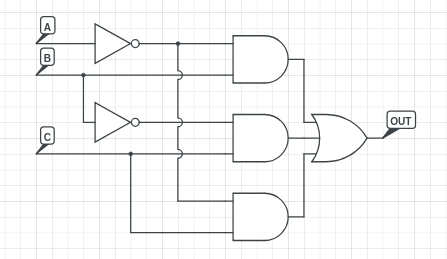
\includegraphics[width=.8\linewidth]{./circsinglitches.jpg}
        \caption{Circuito utilizado de mayor costo.}
        \label{fig:circuito-sin-glitches}
    \end{minipage}
\end{figure}



